% begin module polar-questions
\begin{frame}
\begin{enumerate}
\item<1-| alert@2>  What if $\theta$ is negative?
\item<1-| alert@3>  What if $r$ is negative?
\item<1-| alert@4>  What if $r$ is $0$?
\end{enumerate}
\begin{columns}[c]
\column{.5\textwidth}
\uncover<2->{
\psset{xunit=2cm, yunit=2cm}
\begin{pspicture}(-0.9, -1.2)(2,0.2) 
\tiny 
%force a boudning box:
%\psline[linecolor=red!1](-0.1, -0.1)(-0.21,0.2)
%\psline[linecolor=red!1](1.1, 0.6)(1.1,0.61)
\psFullDotBlue{0}{0}

%Calculator input: plotCurve{}(1/10 \cos{}t, 1/10 \sin{}t, 0, -3/4 \pi)
\parametricplot[arrows=->, linecolor=\psColorGraph, plotpoints=100]{0} {-2.35619} {t 57.29578 mul cos 0.3000000 mul t 57.29578 mul sin 0.3000000 mul }
\rput[t] (0,-0.1){$O$}
\rput[l](0.3, -0.2){$\theta=-\frac{3\pi}{4}$}

\psline{->}(0,0)(2,0)
\psline[linecolor=blue](0,0)(-0.707106781, -0.707106781)
\psFullDotBlue{-0.707106781}{-0.707106781}
\rput[tl](-0.6, -0.7){$\begin{array}{l}(\rho,\theta)=\left(1, -\frac{3\pi}{4}\right)\\ (x,y)=\left(-\frac{\sqrt{2}}2, -\frac{\sqrt{2}}2 \right) \end{array}$}
\end{pspicture} 
}

\uncover<3->{
\psset{xunit=2cm, yunit=2cm}
\begin{pspicture}(-0.9, -1.5)(1.7,0.8) 
\tiny 
%force a boudning box:
%\psline[linecolor=red!1](-0.1, -0.1)(-0.21,0.2)
%\psline[linecolor=red!1](1.1, 0.6)(1.1,0.61)
\psFullDotBlue{0}{0}

\parametricplot[arrows=->, linecolor=\psColorGraph, plotpoints=100]{0} {0.523598776 } {t 57.29578 mul cos 0.3000000 mul t 57.29578 mul sin 0.3000000 mul }
\parametricplot[arrows=->, linecolor=brown, plotpoints=100]{0} {3.665191429 } {t 57.29578 mul cos 0.25 mul t 57.29578 mul sin 0.25 mul }

\rput[t] (0,-0.1){$O$}

\psline{->}(0,0)(1,0)
\psline[linecolor=blue](0,0)(0.866025404, 0.5)
\psFullDotBlue{0.866025404}{0.5}
\rput[tl](-0.75, -0.5){
$(-\rho, \theta)$
}
\psFullDotBlue{-0.866025404}{-0.5}
\psline[linecolor=blue, linestyle=dashed](0,0) (-0.866025404,-0.5)
\rput[tl](0.6, 0.7){$(\rho, \theta) $}
\end{pspicture} 
}
%\ \uncover<2->{%
%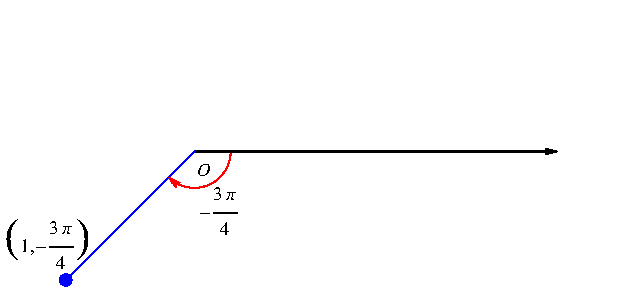
\includegraphics[height=3cm]{polar-curves/pictures/11-03-ex1b.pdf}%
%}%
%\ \uncover<3->{%
%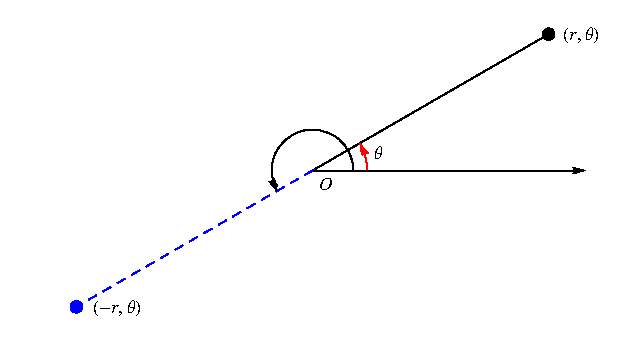
\includegraphics[height=3cm]{polar-curves/pictures/11-03-negativer.pdf}%
%}%
\column{.5\textwidth}
\begin{enumerate}
\item<2-| alert@2>  Positive angles $\theta$ are measured in the counterclockwise direction from $O$.  Negative angles are measured in the clockwise direction.
\item<3-| alert@3>  Points with polar coordinates $(-r, \theta)$ and $(r, \theta)$ lie on the same line through $O$ and at the same distance from $O$, but on opposite sides.
\item<4-| alert@4>  If $r = 0$, then $(r, \theta) = P = O$ for all values of $\theta$.
\end{enumerate}
\end{columns}
\end{frame}
% end module polar-questions
